\documentclass{book}

% IBM Plex Sans Font
\usepackage[sfdefault]{plex-sans}

\usepackage{fancyhdr}
\usepackage{titlesec}

\usepackage{graphicx}

\pagestyle{fancy}

\title{
    \huge{The unofficial ES-2-500 Manual}
    \\
    \vspace{2 mm}
    \small{A 7 1/4" Gauged Electric Railroad Locomotive}
}

\author{Jared Dunbar}

\begin{document}

\maketitle

\tableofcontents

\newpage

\chapter{Overview}

The ES-2-500 is a dual axle electric locomotive with a 500 watt, 24 volt electric motor. The top speed is somewhere between 5 and 8 miles per hour. It comes with a basic 2.4GHz radio control that allows the operator to remotely operate the locomotive from within a decent range, or while riding the locomotive. The locomotive uses regenerative braking to provide stopping power.

\chapter{Operation}

Operation of the ES-2-500 is relatively trivial.

\section{Starting the locomotive}

\begin {enumerate}
    \item {Disconnect the charging cable if it is connected}
    \item {Insert the key into the keyswitch if it has been removed}
    \item {While pushing in the key, turn the key switch clockwise by 90 degrees}
    \item {Turn on the RC controller by pushing the on-off toggle to the left}
\end {enumerate}

\section{Shutting down the locomotive}

\begin{enumerate}
    \item {Turn off the RC controller}
    \item {Turn the key switch counterclockwise by 90 degrees}
    \item {Optionally, remove the key to prevent unauthorized usage}
    \item {Optionally, connect the charging cable}
\end {enumerate}

\section{Riding the locomotive}

When riding any 7 1/4" or 7 1/2" gauge equipment, it is critically important to keep arms and legs close to the center of the train. Do not try to reach out and grab things, as you could cause a derailment. Try to sit centered on the locomotive as though sitting on a horse's saddle. I would highly recommend sitting on a sweatshirt or a towel to make the ride a little smoother.

\section{Controlling the locomotive}

To move the locomotive back and forth, very gently turn the wheel forwards or backwards.
To stop moving, return the wheel to the central position. The locomotive will stop automatically.

\section{Pairing the locomotive in a Multiple-Unit (MU) configuration}

\begin {enumerate}
    \item {Turn on the controller you would like to use as the radio control for the locomotives. Be sure to turn off any other controllers in range.}
    \item {Turn on all locomotives following the start-up procedure, then press the "SW" (pairing) button on the radio receiver in the cab}
    \item {Continue to pair all locomotives by putting them in pairing mode and leaving the controller on}
\end {enumerate}

\chapter{Maintenence}

The most critical maintenence is charging the batteries on a regular basis. When you are not using the locomotive, charging the locomotive is important.
\par\vspace{3mm}
After that, the manufacturer suggested a 6 month regimen of lubricating the chains with motorcycle chain lubricant.

\chapter{Electrical and Mechanical Information}

The ES-2-500 uses a pair of Group 24 12V batteries. At full charge, they are about 25.1 volts.

\par\vspace{3mm}
The motor is a MY1020 and is a 24V, 500W electric motor. It provides roughly 0.7 HP and is geared down from 11:35 between the motor and the jackshaft, and then a further 15:35 between the jackshaft and each of the driven axles. All four wheels are driven by the motor.

\par\vspace{3mm}
In Figure 4.1, the connectors for the lighting circuit were erroneously ommited.

\begin{figure}[h]
    \centering
    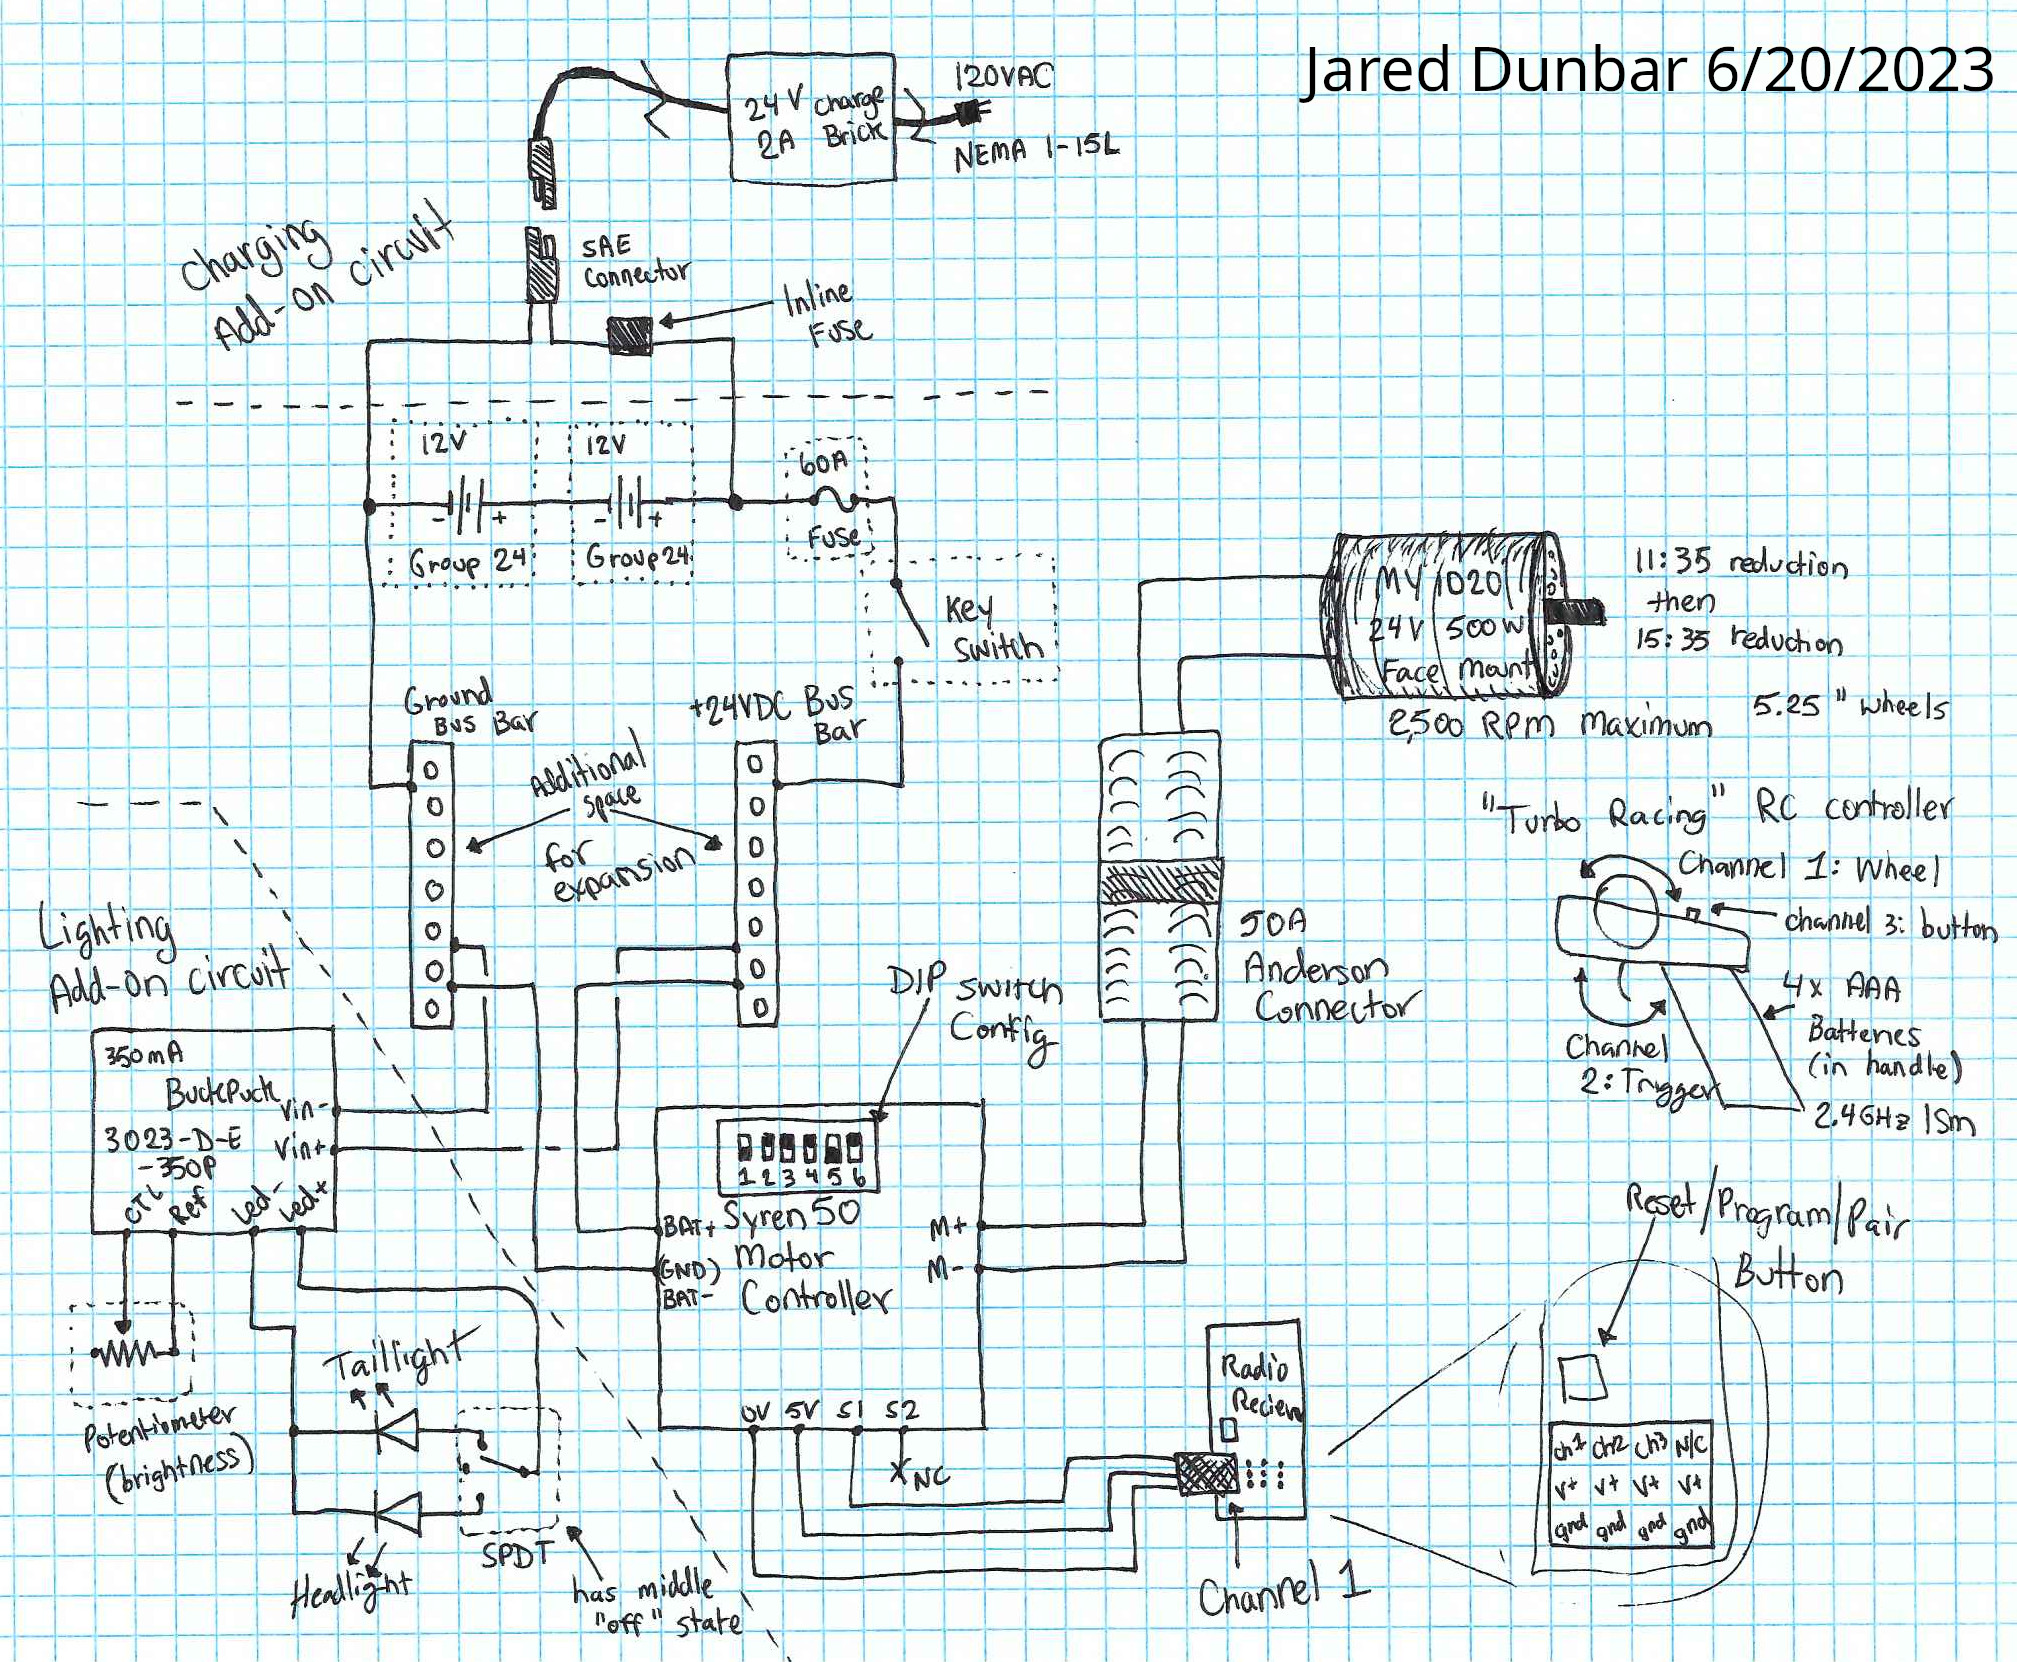
\includegraphics[width=1\textwidth]{schematic.jpg}
    \caption{Typical Electrical Diagram of the ES-2-500, including Charging add-on circuit and Lighting add-on circuit}
\end{figure}


\chapter {Future Plans}

I have various things that I would like to add/modify about this locomotive.
\par\vspace{3mm}
In no particular order:

\begin{itemize}
    \item {Replace the motor and motor controller with a brushless DC motor and controller}
    \item {Replace the RC controller with a custom Atmel-based control, plus 900MHz ISM-band radio for longer range}
    \item {Add a horn}
    \item {Add an air brake system so that it may be utilized with cars with air brakes for additonal safety}
    \item {Add additonal ditch lights and other lights}
    \item {Add current/power/voltage monitoring circuitry}
    \item {Add a spedometer}
    \item {Add an electronic braking system that uses the motor and rotary encoders to prevent rolling}
    \item {Maintian reverse-compatibility with old RC system for MU compatibility with other ES-2-500's}
\end{itemize}

\chapter{Appendix}
\section{RC Controller documentation}

\begin{figure}[h]
    \centering
    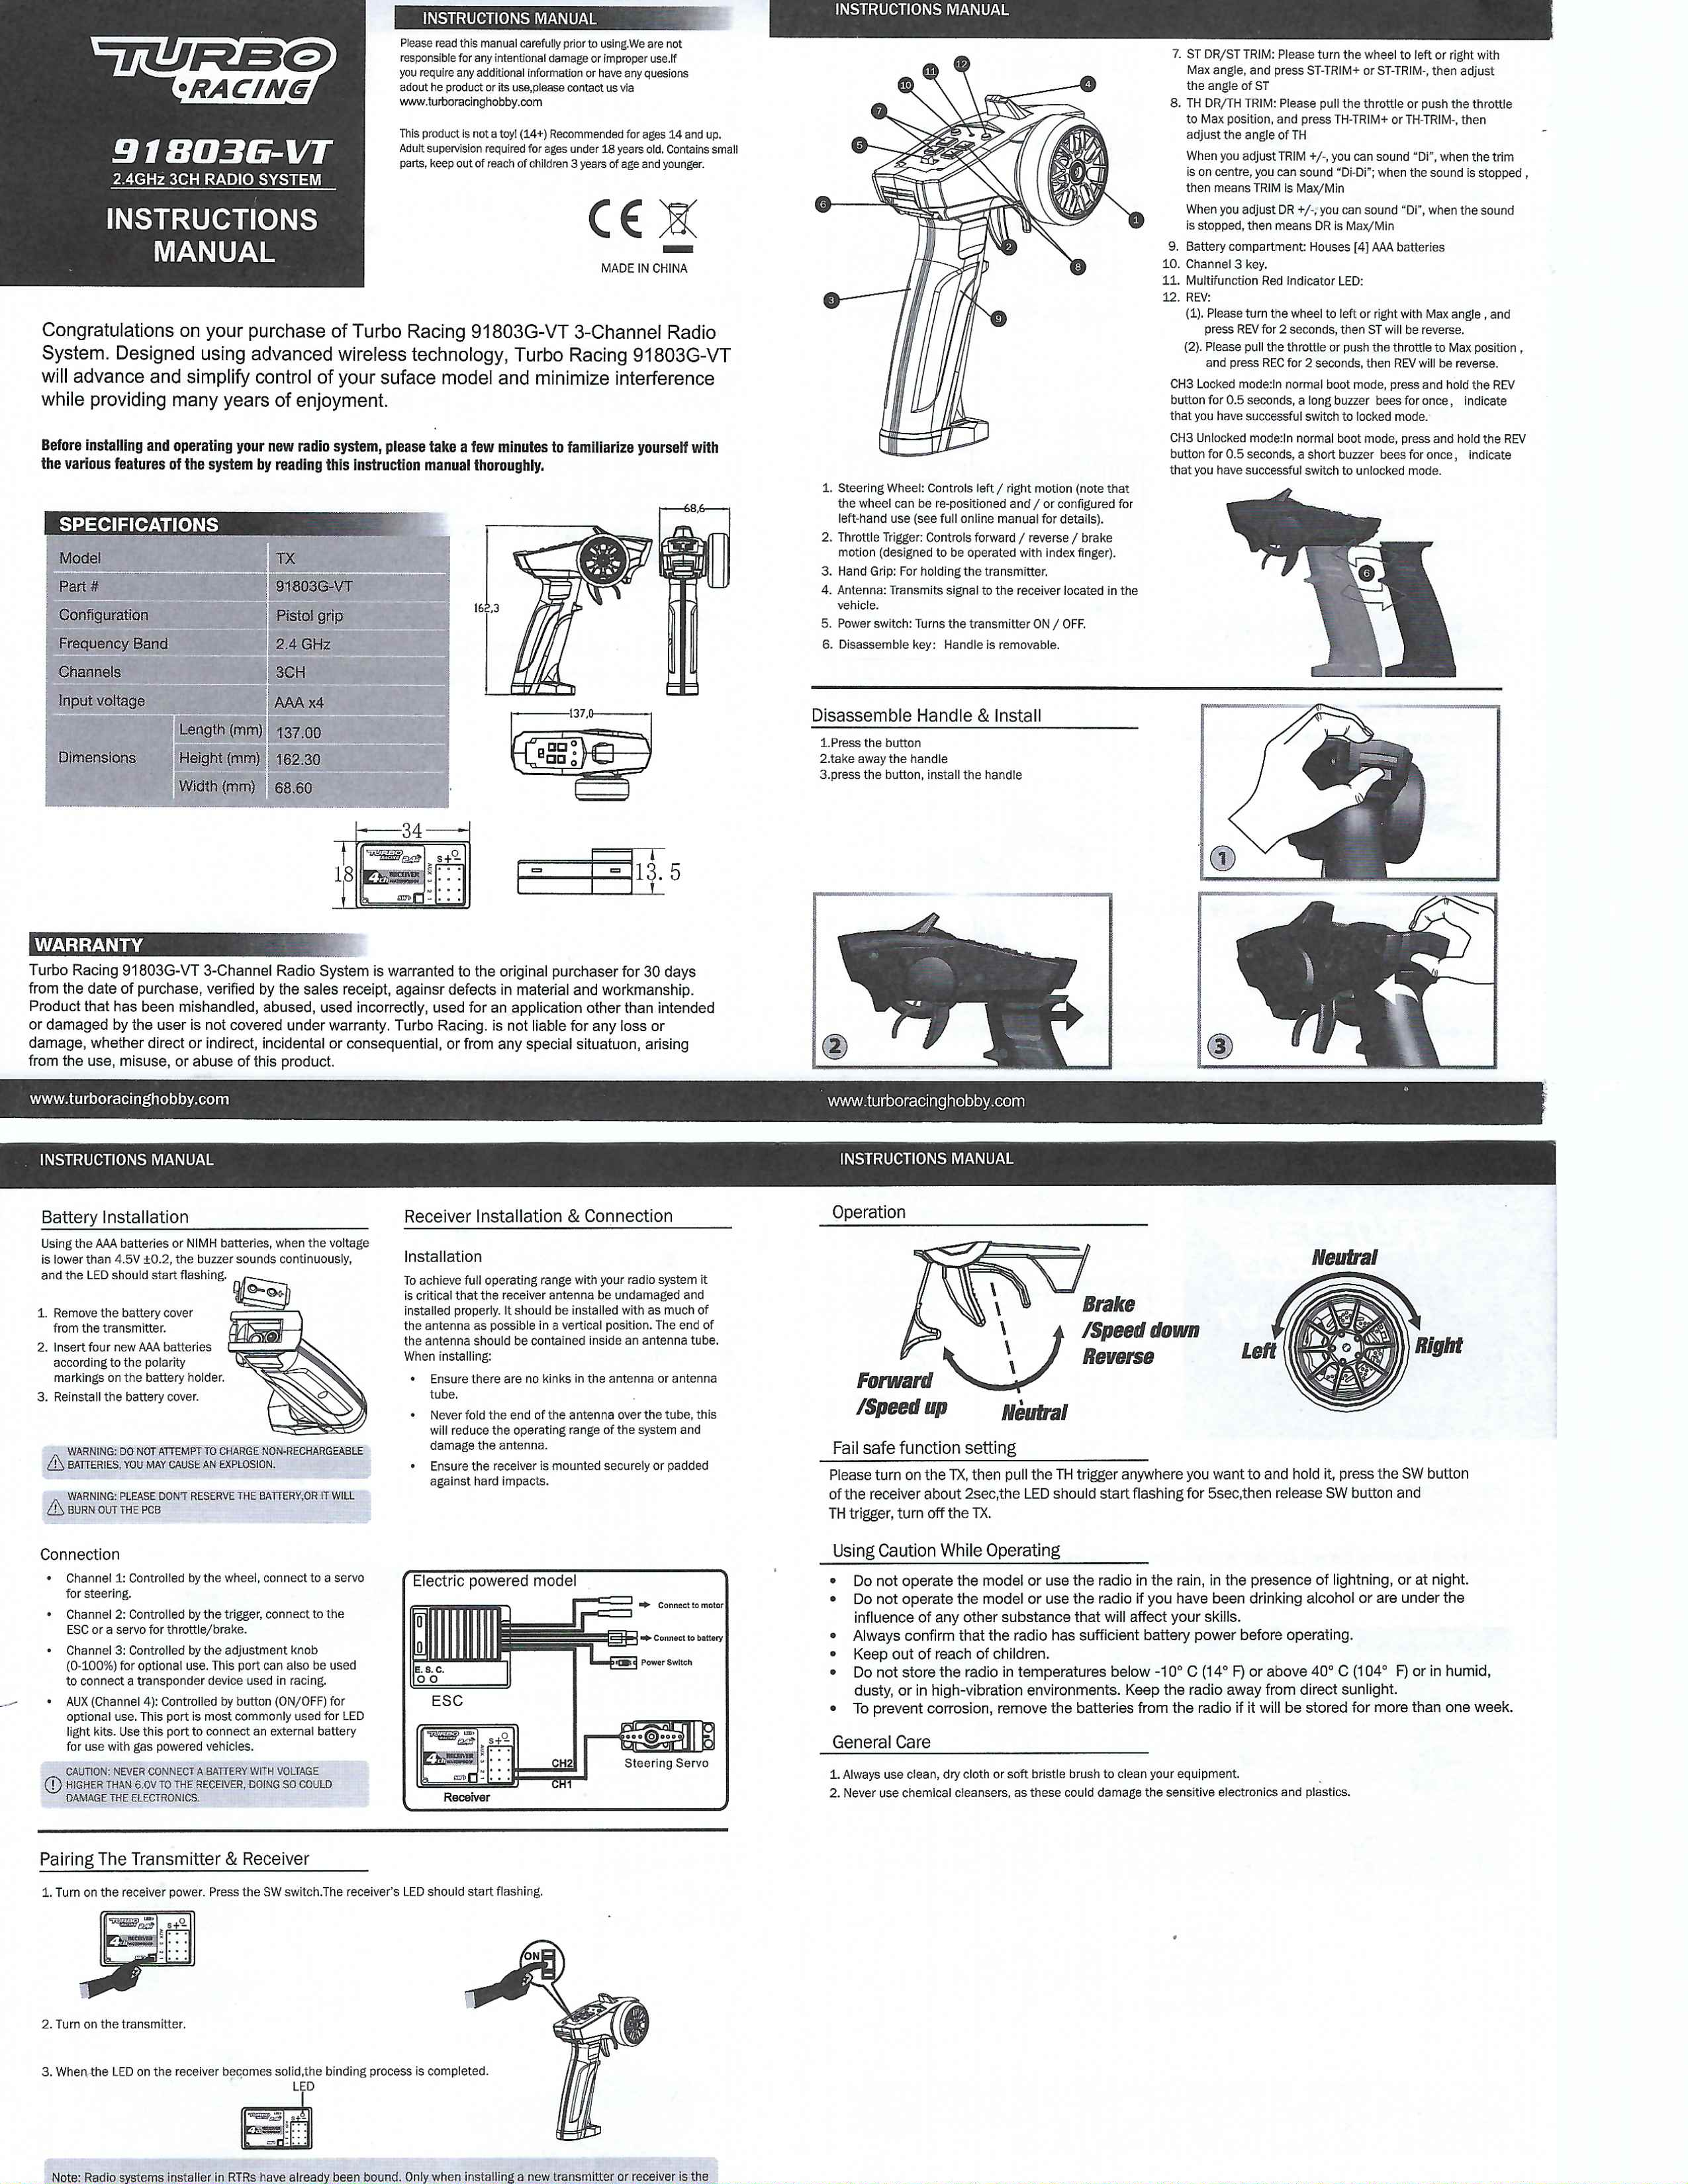
\includegraphics[width=1\textwidth]{controller.jpg}
    \caption{Manufacturer's documentation for the RC controller}
\end{figure}

\end{document}